Osciloscopul va fi format din 3 parti: Logica de intrare, Memoria esantioanelor si logica de iesire.

\begin{figure}[h]
\centering
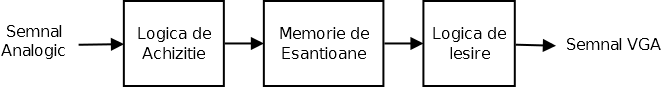
\includegraphics[width=320pt]{block_diagram}
\caption{Schema Block}
\label{fig:block_diagram}
\end{figure}

\paragraph{}
Propunem o implementare in limbaj de descriere hardware a unui osciloscop digital ce poate fi sintetizat pe o placa \textbf{FPGA Basys 2 (Spartan 3E)}. Pentru esantionarea semnalului de intrare vom folosi un convertor analog digital. Vom realiza un protocol de comunicare intre convertor si placuta FPGA astfel incat sa fie usor de schimbat cu alt convertor de exemplu. Frecventa de esantionare a semnalului o vom controla de la switch-uri sau butoane. 
\paragraph{}
Dispunem de o placuta \textbf{CEREBOT II}, placuta care are integrat un  \textbf{convertor AD/10 biti} pe care il putem folosi. Pentru afisarea datelor vom folosi un monitor cu intrare \textbf{VGA}. Placuta Basys 2 dispune de o iesire VGA integrata. Controlul osciloscopului se va face cu ajutorul butoanelor si switch-urilor placutei Basys 2.
\paragraph{}
Ideea de baza a dispozitivului e sa esantioneze un semnal la un interval de timp modificabil si sa salveze pentru fiecare perioada de timp o valoare care reprezinta amplitudinea semnalului de intrare. Dimensiunea intervalului de timp monitorizat este prestabilit sau se poate controla de la switch-uri/butoane. De fiecare data cand intervalul este baleiat vom trimite datele spre controller-ul VGA spre a fi afisate. 
\paragraph{}
Pentru afisarea graficului putem utiliza interpolare spline liniara intre valorile succesive ale amplitudinii semnalului. Cel mai probabil vom avea nevoie de o matrice bidimensionala de pixeli (framebuffer) in care vom desena forma de unda a semnalului de intrare.